\documentclass[11pt,a4paper]{article}
\usepackage[T1]{fontenc}
\usepackage{lmodern,microtype}
\usepackage[margin=25mm]{geometry}
\usepackage{amsmath,amssymb,amsthm,mathtools}
\usepackage{booktabs,array,enumitem,xcolor,fancyhdr,needspace}
\usepackage{tikz,listings}
\usepackage[hypertexnames=false,colorlinks=true,linkcolor=blue!45!black,citecolor=blue!45!black,urlcolor=blue!45!black]{hyperref}
\setlength{\emergencystretch}{3em}
\setlength{\parskip}{0.25em}
\setlist{topsep=3pt,itemsep=3pt}
\pagestyle{fancy}\fancyhf{}
\fancyhead[L]{\small Nonconvexity of Robin eigenvalues under dilation}
\fancyhead[R]{\small Research manuscript}
\fancyfoot[C]{\thepage}
\setlength{\headheight}{14pt}
\newtheorem{theorem}{Theorem}[section]
\newtheorem{lemma}[theorem]{Lemma}
\newtheorem{proposition}[theorem]{Proposition}
\newtheorem{corollary}[theorem]{Corollary}
\theoremstyle{definition}\newtheorem{definition}[theorem]{Definition}
\theoremstyle{remark}\newtheorem{remark}[theorem]{Remark}
\newcommand{\CM}{\mathrm{CM}}
\newcommand{\dd}{\,\mathrm d}
\DeclareMathOperator{\Tr}{Tr}
\DeclareMathOperator{\interior}{int}
\lstset{basicstyle=\ttfamily\scriptsize,breaklines=true,columns=fullflexible,
  keepspaces=true,showstringspaces=false,frame=single,rulecolor=\color{black!25},
  xleftmargin=3pt,xrightmargin=3pt,aboveskip=8pt,belowskip=8pt}
\title{Failure of Convexity under Dilation\\for the First Robin Eigenvalue\\[5pt]
\large A connected-domain answer to a question of\\Keady and Wiwatanapataphee}
\author{Keio Research Notes}
\date{31 October 2026}
\hypersetup{pdftitle={Failure of Convexity under Dilation for the First Robin Eigenvalue},pdfauthor={Keio Research Notes},pdfsubject={Connected-domain counterexamples to the general-domain dilation question in Keady and Wiwatanapataphee (2018)}}
\begin{document}
\maketitle
\begin{abstract}
For the boundary condition $\beta\partial_\nu u+u=0$, with
$\beta>0$ fixed, we construct bounded connected simply connected
domains on which the first Robin eigenvalue is not convex as a
function of the dilation factor. This gives a negative answer to
the general-domain complete-monotonicity question posed by Keady
and Wiwatanapataphee in 2018. The construction joins an $8\times2$
rectangle and a $3\times3$ square by a thin passage. The two
chambers exchange which one has the smaller first eigenvalue.
At three specified rational scales, exact rational arithmetic
certifies a strict midpoint defect exceeding $1/16000$ for their
minimum. A direct variational argument transfers this defect to
every sufficiently thin positive-width passage. The same fixed
planar domain works for every $\beta>0$, and Cartesian products
give counterexamples in every dimension at least two, also after
unit-volume normalization. We further give an open parameter
family in which reversal of the small- and large-scale ordering
forces failure of complete monotonicity. All numerical-looking
inequalities in the main construction are certified by finite
rational calculations. The thin-passage technique is established;
the contribution examined here is its application through chamber
ground-state switching to the original dilation question.
\end{abstract}

\section{The original question and the counterexample}

For a bounded Lipschitz domain $D\subset\mathbb R^d$, write
$\lambda_1(D;\beta)$ for the first eigenvalue of
\begin{equation}\label{eq:boundary}
 -\Delta u=\lambda u\quad\hbox{in }D,\qquad
 \beta\partial_\nu u+u=0\quad\hbox{on }\partial D,
 \qquad \beta>0.
\end{equation}
The Robin parameter is constant on the entire exterior boundary.
A smooth function $f:(0,\infty)\to\mathbb R$ is completely
monotone if $(-1)^n f^{(n)}\ge0$ for every integer $n\ge0$.
In particular, every such function is convex.

Keady and Wiwatanapataphee \cite{KW2018}, Section~6, printed
pages~924--925, ask whether the complete monotonicity of
$s\mapsto\lambda_1(sD;0)$ persists for positive $\beta$, including
when $D$ is a rectangle. Their general setting on printed
page~911 is a bounded simply connected domain with piecewise
$C^1$ boundary; convexity of the domain is not assumed. The
following theorem answers the arbitrary-domain assertion
negatively in precisely that geometric class. It makes no claim
of a counterexample among rectangles or convex domains.

Set
\begin{align}
 A&=(-4,4)\times(-1,1),&
 B&=(6,9)\times(-3/2,3/2),\label{eq:chambers}\\
 T_\varepsilon&=(4,6)\times(-\varepsilon,\varepsilon),&
 \Omega_\varepsilon
 &=\interior(\overline A\cup\overline T_\varepsilon\cup\overline B),
 \qquad 0<\varepsilon<1/4.\label{eq:domain}
\end{align}
The interior-of-the-union convention includes the open attachment
windows. Thus $\Omega_\varepsilon$ is a connected simply connected
Lipschitz polygon, with area $25+4\varepsilon$.

\begin{figure}[ht]
\centering
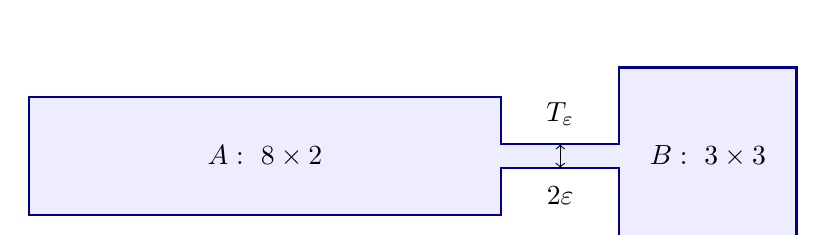
\begin{tikzpicture}[x=0.75cm,y=0.75cm]
 \fill[blue!7] (-4,-1)--(4,-1)--(4,-0.2)--(6,-0.2)--(6,-1.5)
 --(9,-1.5)--(9,1.5)--(6,1.5)--(6,0.2)--(4,0.2)--(4,1)--(-4,1)--cycle;
 \draw[thick,blue!55!black] (-4,-1)--(4,-1)--(4,-0.2)--(6,-0.2)--(6,-1.5)
 --(9,-1.5)--(9,1.5)--(6,1.5)--(6,0.2)--(4,0.2)--(4,1)--(-4,1)--cycle;
 \node at (0,0) {$A:\ 8\times2$};
 \node at (7.5,0) {$B:\ 3\times3$};
 \node[above] at (5,0.35) {$T_\varepsilon$};
 \draw[<->] (5,-0.2)--(5,0.2);
 \node[below] at (5,-0.35) {$2\varepsilon$};
\end{tikzpicture}
\caption{The explicit family of connected domains. The passage width
is schematic: the theorem proves the result for all sufficiently
small positive $\varepsilon$, without specifying a numerical threshold.}
\label{fig:domain}
\end{figure}

\begin{theorem}[A strict failure of dilation convexity]\label{thm:main}
Let
\begin{equation}\label{eq:scales}
 s_- =\frac{1657}{1000},\qquad
 s_0 =\frac{1667}{1000},\qquad
 s_+ =\frac{1677}{1000}.
\end{equation}
There exists $\varepsilon_0>0$ such that, for every
$0<\varepsilon<\varepsilon_0$ and every $\beta>0$,
\begin{equation}\label{eq:main-gap}
 \lambda_1(\beta s_0\Omega_\varepsilon;\beta)
 -\frac{\lambda_1(\beta s_-\Omega_\varepsilon;\beta)
       +\lambda_1(\beta s_+\Omega_\varepsilon;\beta)}2
 >\frac1{32000\beta^2}.
\end{equation}
Consequently, $s\mapsto\lambda_1(s\Omega_\varepsilon;\beta)$
is not convex and is not completely monotone. The domain can be
chosen independently of $\beta$.
\end{theorem}

\begin{theorem}[Every dimension and fixed volume]\label{thm:dimensions}
For every integer $d\ge2$ there is a bounded connected simply
connected Lipschitz polyhedral domain $D_d\subset\mathbb R^d$
such that $s\mapsto\lambda_1(sD_d;\beta)$ fails convexity for
every $\beta>0$. One may require $|D_d|=1$.
\end{theorem}

The proof has two distinct tasks. First we certify a strict
finite-value inequality for a minimum of two explicit interval
spectra. Then we realize that minimum as a limit of the first
eigenvalues of connected domains. The latter step is a standard
thin-passage idea, for which we give a complete variational proof.
The former supplies the particular obstruction to the dilation
property. Section~\ref{sec:prior} distinguishes this result from
nearby literature and records the limits of the priority claim.

\section{Interval coordinates and the scaling identities}

It is useful to distinguish the reciprocal boundary conventions.
For $\alpha>0$, define
\begin{align}
 q_{D,\alpha}[u]&=\int_D|\nabla u|^2\dd x
          +\alpha\int_{\partial D}|\Tr u|^2\dd\sigma,
 &u&\in H^1(D),\label{eq:form}\\
 \Lambda(D;\alpha)&=\inf_{u\ne0}
             \frac{q_{D,\alpha}[u]}{\|u\|_{L^2(D)}^2}.
 &&\label{eq:rayleigh}
\end{align}
Thus $\Lambda(D;\alpha)$ uses $\partial_\nu u+\alpha u=0$,
and $\lambda_1(D;\beta)=\Lambda(D;1/\beta)$.
Changing variables in the Rayleigh quotient gives
\begin{equation}\label{eq:scale}
 \lambda_1(sD;\beta)=s^{-2}\Lambda(D;s/\beta),
 \qquad
 \lambda_1(tD;\beta)
 =\beta^{-2}\lambda_1((t/\beta)D;1).
\end{equation}
In particular, the parameter transfer in Theorem~\ref{thm:main}
is exact and involves no uniform-in-$\beta$ limiting argument.

For $y>0$, let $\mu(y)>0$ be determined by
\begin{equation}\label{eq:mu}
 y\mu(y)=\arctan\frac1{\mu(y)},
 \quad\hbox{equivalently}\quad
 H_y(\mu(y))=0,
 \qquad H_y(x)=yx+\arctan x-\frac\pi2.
\end{equation}
Since $H_y'(x)=y+(1+x^2)^{-1}>0$, there is a unique positive
solution. The implicit function theorem shows that $\mu$ is
real analytic. Also
\begin{equation}\label{eq:mu-monotone-bound}
 \mu'(y)=-\frac{\mu(y)}{y+(1+\mu(y)^2)^{-1}}<0,
 \qquad 0<\mu(y)<\frac\pi{2y}.
\end{equation}

\begin{lemma}[The rectangle formula]\label{lem:rectangle}
For a rectangle with half-side lengths $a,b>0$,
\begin{equation}\label{eq:rectangle}
 \lambda_1\bigl(s((-a,a)\times(-b,b));1\bigr)
 =\mu(as)^2+\mu(bs)^2.
\end{equation}
Translations of the rectangle do not change this formula.
\end{lemma}
\begin{proof}
On the interval $(-y,y)$, the positive even ground state is
$\cos(\mu(y)x)$; the boundary condition is
$\mu(y)\tan(y\mu(y))=1$ with $0<y\mu(y)<\pi/2$.
This is equivalent to \eqref{eq:mu}. The one-dimensional
variational characterization gives a lower bound by $\mu(y)^2$
for each slice. Apply that bound separately to the two coordinate
directions and integrate. The product of the two cosine ground
states attains the resulting lower bound, proving the formula.
\end{proof}

Applied to \eqref{eq:chambers}, the formula gives two analytic
branches and their minimum:
\begin{equation}\label{eq:envelope}
 a(s)=\mu(s)^2+\mu(4s)^2,\qquad
 b(s)=2\mu(3s/2)^2,\qquad F(s)=\min\{a(s),b(s)\}.
\end{equation}
These are exactly the first eigenvalues of the two scaled
chambers and their disconnected union. The union is only an
intermediate model; the final examples have a positive-width
passage.

\section{Designing an order reversal}
\label{sec:design}

The auxiliary design problem is to make two elementary chamber
spectra exchange their order as the scale changes. This can be
done for every nonsquare rectangle.

\begin{lemma}[Endpoint asymptotics]\label{lem:asymptotics}
The interval function satisfies
\begin{equation}\label{eq:asymptotics}
 \mu(y)^2\sim\frac1y\quad(y\downarrow0),\qquad
 \mu(y)^2\sim\frac{\pi^2}{4y^2}\quad(y\to\infty).
\end{equation}
\end{lemma}
\begin{proof}
The function $x\mapsto\arctan(1/x)/x$ decreases continuously
from $+\infty$ to $0$. Hence its inverse tends to $+\infty$
as $y\downarrow0$, and to $0$ as $y\to\infty$. In the first
limit, \eqref{eq:mu} gives
$y\mu(y)^2=\mu(y)\arctan(1/\mu(y))\to1$.
In the second it gives $y\mu(y)\to\pi/2$.
\end{proof}

\begin{proposition}[An open family of competing chambers]
\label{prop:competing}
Let $a,b>0$ with $a\ne b$, and choose $c$ in the nonempty interval
\begin{equation}\label{eq:c-range}
 \frac{\sqrt2\,ab}{\sqrt{a^2+b^2}}
       <c<\frac{2ab}{a+b}.
\end{equation}
Set
\[
 R(s)=\mu(as)^2+\mu(bs)^2,\qquad Q(s)=2\mu(cs)^2.
\]
Then $R(s)<Q(s)$ for all sufficiently small $s>0$, while
$R(s)>Q(s)$ for all sufficiently large $s$. The function
$\min\{R,Q\}$ is not real analytic on $(0,\infty)$ and is
not completely monotone.
\end{proposition}
\begin{proof}
The asymptotic coefficients in Lemma~\ref{lem:asymptotics} are
\begin{align*}
 R(s)&\sim\frac{a^{-1}+b^{-1}}s,&Q(s)&\sim\frac{2}{cs}
 &&(s\downarrow0),\\
 R(s)&\sim\frac{\pi^2}{4s^2}(a^{-2}+b^{-2}),&
 Q(s)&\sim\frac{\pi^2}{4s^2}\frac2{c^2}
 &&(s\to\infty).
\end{align*}
The two strict inequalities in \eqref{eq:c-range} are precisely
the inequalities that reverse these orderings. The interval is
nonempty because
$2(a^2+b^2)>(a+b)^2$ when $a\ne b$.

If the minimum were real analytic, its agreement with $R$ on
a nonempty open interval would, by the real-analytic identity
theorem, force agreement on all of $(0,\infty)$. This contradicts
the opposite strict ordering at large scales. Complete
monotonicity implies real analyticity by the Laplace-transform
representation, so it is excluded as well; see \cite{SSV2012}.
\end{proof}

For $(a,b,c)=(4,1,3/2)$, the comparison reduces to
\begin{equation}\label{eq:ordering}
 \frac54<\frac43,
 \qquad \frac{17}{64}>\frac29.
\end{equation}
The small-scale coefficients are the perimeter-to-area ratios
of the two chambers. The large-scale coefficients are their
first Dirichlet eigenvalues divided by $\pi^2$.

Order reversal alone gives a qualitative obstruction to complete
monotonicity. It does not by itself prove failure of convexity:
two analytic branches might meet to higher order. The next
section supplies a strict midpoint witness, which is the only
finite calculation used in the stronger theorem.

\section{A rational certificate for the midpoint defect}
\label{sec:certificate}

\begin{proposition}[Exact finite witness]\label{prop:gap}
For $F$ in \eqref{eq:envelope} and the scales in
\eqref{eq:scales},
\begin{equation}\label{eq:exact-gap}
 F(s_0)-\frac{F(s_-)+F(s_+)}2
 >\frac{674670894519}{10^{16}}>\frac1{16000}.
\end{equation}
\end{proposition}

\begin{proof}
We give finite rational bounds for the six interval roots that
are needed. For $0<x<1$, define
\[
 S_m(x)=\sum_{k=0}^m\frac{(-1)^k x^{2k+1}}{2k+1}.
\]
The alternating-series estimate gives
\begin{equation}\label{eq:atan-bounds}
 S_{2n+1}(x)<\arctan x<S_{2n}(x).
\end{equation}
Using Machin's identity
$\pi=16\arctan(1/5)-4\arctan(1/239)$, put
\begin{align}
 p_-&=16S_{21}(1/5)-4S_{20}(1/239),\notag\\
 p_+&=16S_{20}(1/5)-4S_{21}(1/239).
 \label{eq:pi-bounds}
\end{align}
Then $p_-<\pi<p_+$. For completeness, Machin's identity follows
by applying the tangent addition formula twice:
$\tan(4\arctan(1/5))=120/119$, and subtracting
$\arctan(1/239)$ gives tangent $1$. The angle lies in
$(0,\pi/2)$, so it is $\pi/4$.

In Table~\ref{tab:roots}, set $\ell_j=n_j/10^8$ and
$u_j=(n_j+1)/10^8$. The last two columns are integer certificates
for the following strictly rational inequalities:
\begin{align}
 10^9\bigl(y_j\ell_j+S_{40}(\ell_j)-p_-/2\bigr)&<U_j<0,
 \label{eq:cert-low}\\
 10^9\bigl(y_ju_j+S_{41}(u_j)-p_+/2\bigr)&>V_j>0.
 \label{eq:cert-high}
\end{align}
They are obtained by substituting the displayed integers into
the finite sums; a complete standard-library rational verifier
is included in Appendix~\ref{app:code}. By
\eqref{eq:atan-bounds}--\eqref{eq:pi-bounds}, these inequalities
imply $H_{y_j}(\ell_j)<0<H_{y_j}(u_j)$. Strict increase of
$H_{y_j}$ therefore proves
\begin{equation}\label{eq:root-brackets}
 \ell_j<\mu(y_j)<u_j\qquad(1\le j\le6).
\end{equation}

\begin{table}[ht]
\centering
\caption{Exact brackets of width $10^{-8}$ for the six roots.
All four numerical columns contain exact rational or integer data.}
\label{tab:roots}
\begin{tabular}{clrrrr}
\toprule
$j$ & Role & $y_j$ & $n_j$ & $U_j$ & $V_j$\\
\midrule
1 & $\mu(s_-)$ & $1657/1000$ & $61515335$ & $-2$ & $21$\\
2 & $\mu(4s_-)$ & $6628/1000$ & $20629921$ & $-72$ & $3$\\
3 & $\mu(s_0)$ & $1667/1000$ & $61258304$ & $-1$ & $21$\\
4 & $\mu(4s_0)$ & $6668/1000$ & $20521733$ & $-17$ & $58$\\
5 & $\mu(3s_0/2)$ & $5001/2000$ & $45682209$ & $-16$ & $17$\\
6 & $\mu(3s_+/2)$ & $5031/2000$ & $45477263$ & $-23$ & $9$\\
\bottomrule
\end{tabular}
\end{table}

At the center, both branches require lower bounds. At the
endpoints, it suffices to bound any one branch from above:
\begin{align*}
 F(s_0)&>\min\{\ell_3^2+\ell_4^2,\,2\ell_5^2\},\\
 F(s_-)&<u_1^2+u_2^2,\qquad
 F(s_+)<2u_6^2.
\end{align*}
There is no assumption about which branch attains the minimum
at either endpoint. Direct integer arithmetic gives
\begin{align*}
 &\min\{\ell_3^2+\ell_4^2,\,2\ell_5^2\}
     -\tfrac12(u_1^2+u_2^2+2u_6^2)\\
 &\hspace{15mm}=\frac{674670894519}{10^{16}}
 =\frac1{16000}+\frac{49670894519}{10^{16}}.
\end{align*}
Both strict comparisons in \eqref{eq:exact-gap} follow.
\end{proof}

The certificate uses no decimal approximation as a premise.
The alternating sums, the Machin bounds, the root enclosures,
and the final comparison are all finite rational statements.
In particular, no numerical crossing location or derivative
estimate is required.

\section{An elementary limit for a thin passage}
\label{sec:neck}

\begin{lemma}[Convergence to the chamber minimum]\label{lem:neck}
For every fixed $\alpha>0$,
\begin{equation}\label{eq:neck-limit}
 \lim_{\varepsilon\downarrow0}\Lambda(\Omega_\varepsilon;\alpha)
 =\min\{\Lambda(A;\alpha),\Lambda(B;\alpha)\}.
\end{equation}
The same statement holds for two fixed rectangles attached at
the centers of facing sides by a straight passage of any fixed
positive length and width $2\varepsilon$.
\end{lemma}

\begin{proof}
We prove both inequalities directly. Compactness is used only
on the two fixed chambers.

\emph{Upper estimate.}
Choose a chamber $D\in\{A,B\}$ and its normalized first Robin
eigenfunction $v$ for the coefficient $\alpha$. Separation of
variables makes $v$ a product of cosine functions, so $v$ and
$\nabla v$ are bounded on the closed rectangle. Let $P$ be the
center of the attachment window. Put
\[
 r_\varepsilon=2\varepsilon,\qquad R_\varepsilon=\sqrt\varepsilon,
 \qquad L_\varepsilon=\log(R_\varepsilon/r_\varepsilon).
\]
For sufficiently small $\varepsilon$, define
\[
 \chi_\varepsilon(x)=
 \begin{cases}
 0,&|x-P|\le r_\varepsilon,\\
 \log(|x-P|/r_\varepsilon)/L_\varepsilon,
       &r_\varepsilon<|x-P|<R_\varepsilon,\\
 1,&|x-P|\ge R_\varepsilon.
 \end{cases}
\]
Its exceptional region has area at most $\pi\varepsilon$, and
polar integration gives
\begin{equation}\label{eq:capacity}
 \int_{\mathbb R^2}|\nabla\chi_\varepsilon|^2\dd x
 =\frac{2\pi}{L_\varepsilon}\longrightarrow0.
\end{equation}
By the product rule and boundedness of $v,\nabla v$, this proves
$\chi_\varepsilon v\to v$ strongly in $H^1(D)$. The trace
operator on the fixed rectangle is continuous, so the boundary
traces converge in $L^2(\partial D)$.

Extend $\chi_\varepsilon v$ by zero to the rest of
$\Omega_\varepsilon$. This extension belongs to
$H^1(\Omega_\varepsilon)$ because it vanishes on a neighborhood
of the entire window. The Rayleigh quotient on the joined
domain tends to $\Lambda(D;\alpha)$. Choosing either chamber
gives
\begin{equation}\label{eq:limsup}
 \limsup_{\varepsilon\downarrow0}\Lambda(\Omega_\varepsilon;\alpha)
 \le\min\{\Lambda(A;\alpha),\Lambda(B;\alpha)\}.
\end{equation}

\emph{The passage cannot retain mass at bounded energy.}
For $f\in H^1(-\varepsilon,\varepsilon)$, the fundamental
theorem of calculus and Cauchy--Schwarz give
\[
 \int_{-\varepsilon}^{\varepsilon}|f(y)|^2\dd y
 \le4\varepsilon|f(\varepsilon)|^2
       +8\varepsilon^2\int_{-\varepsilon}^{\varepsilon}|f'(y)|^2\dd y.
\]
Apply this to transverse slices of $u\in H^1(\Omega_\varepsilon)$
and integrate along the passage. Its top side is part of the
exterior Robin boundary. Thus
\begin{equation}\label{eq:neck-mass}
 \int_{T_\varepsilon}|u|^2\dd x
 \le\left(\frac{4\varepsilon}{\alpha}+8\varepsilon^2\right)
           q_{\Omega_\varepsilon,\alpha}[u].
\end{equation}
The positive Robin coefficient on the lateral boundary is
essential in this estimate.

\emph{Lower estimate.}
Choose a sequence $\varepsilon\downarrow0$ realizing the lower
limit of the eigenvalues, and normalized first eigenfunctions
$u_\varepsilon$. The upper estimate bounds their energies.
Their restrictions to $A$ and $B$ are bounded in the two fixed
$H^1$ spaces. After passing to a subsequence, these restrictions
converge weakly in $H^1$ and strongly in $L^2$ to $u_A,u_B$.
Equation~\eqref{eq:neck-mass} implies
\begin{equation}\label{eq:mass-one}
 \|u_A\|_{L^2(A)}^2+\|u_B\|_{L^2(B)}^2=1.
\end{equation}
For $\delta>0$, omit from each chamber boundary the part in
the radius-$\delta$ disk about its attachment point $P_D$.
For all sufficiently small $\varepsilon$, the remaining fixed
boundary portions belong to $\partial\Omega_\varepsilon$.
Weak continuity of the trace on each fixed chamber and weak
lower semicontinuity yield
\begin{align*}
 \liminf_{\varepsilon\downarrow0}
 q_{\Omega_\varepsilon,\alpha}[u_\varepsilon]
 \ge\sum_{D\in\{A,B\}}\biggl(
 \int_D|\nabla u_D|^2\dd x
 +\alpha\int_{\partial D\setminus B(P_D,\delta)}
             |\Tr u_D|^2\dd\sigma\biggr).
\end{align*}
Let $\delta\downarrow0$. The limiting omitted sets are single
points of zero boundary measure. Monotone convergence, the
Rayleigh principle, and \eqref{eq:mass-one} give
\begin{align*}
 \liminf_{\varepsilon\downarrow0}\Lambda(\Omega_\varepsilon;\alpha)
 &\ge q_{A,\alpha}[u_A]+q_{B,\alpha}[u_B]\\
 &\ge\min\{\Lambda(A;\alpha),\Lambda(B;\alpha)\}.
\end{align*}
Together with \eqref{eq:limsup}, this proves the limit. The
argument depends only on fixed rectangular chambers, side-center
attachments, and a fixed positive passage length, proving the
last assertion as well.
\end{proof}

\section{Transfer to connected domains and all dimensions}
\label{sec:transfer}

\begin{proof}[Proof of Theorem~\ref{thm:main}]
By \eqref{eq:scale}, Lemma~\ref{lem:neck}, and
Lemma~\ref{lem:rectangle}, for every fixed $s>0$,
\begin{equation}\label{eq:pointwise}
 f_\varepsilon(s):=\lambda_1(s\Omega_\varepsilon;1)
 \longrightarrow F(s).
\end{equation}
Let $\eta=1/16000$. Proposition~\ref{prop:gap} gives a limiting
midpoint defect greater than $\eta$. Convergence at the three
fixed scales permits the simultaneous estimates
\[
 |f_\varepsilon(s_j)-F(s_j)|<\eta/4,
 \qquad j\in\{-,0,+\},
\]
for all $0<\varepsilon<\varepsilon_0$ after choosing one
$\varepsilon_0>0$. The total error in the midpoint defect is
less than $\eta/2$. Consequently
\begin{equation}\label{eq:planar-gap}
 f_\varepsilon(s_0)-\frac{f_\varepsilon(s_-)+f_\varepsilon(s_+)}2
 >\eta/2=\frac1{32000}.
\end{equation}
This violates the defining midpoint inequality for convexity.
Finally, the second identity in \eqref{eq:scale} multiplies this
gap by $\beta^{-2}$ and the three scales by $\beta$, giving
\eqref{eq:main-gap}. No convergence of derivatives, unidentified
eigenvalue crossing, or conjectural regularity is used.
\end{proof}

The assertion ``for all sufficiently small positive
$\varepsilon$'' is an unconditional existence statement about
actual connected polygons. The proof does not specify a numerical
value of $\varepsilon_0$, and it does not certify a selected
decimal passage width. Such an explicit threshold would require
a quantitative refinement of Lemma~\ref{lem:neck}, but is not
needed for the stated counterexample.

\begin{proof}[Proof of Theorem~\ref{thm:dimensions}]
Fix any $\varepsilon$ satisfying Theorem~\ref{thm:main}.
The case $d=2$ is already proved. For $d\ge3$, set
\[
 L=1000d,\qquad
 D_{d,\varepsilon}=\Omega_\varepsilon\times(-L,L)^{d-2}.
\]
This is a bounded connected simply connected Lipschitz
polyhedral domain. The first eigenvalue on a Cartesian product
is the sum of the first eigenvalues on its factors: the lower
bound follows by applying the variational inequality on slices,
and the product of ground states attains it. Hence
\[
 \lambda_1(sD_{d,\varepsilon};1)
 =f_\varepsilon(s)+(d-2)\mu(sL)^2.
\]
Since $\mu$ is decreasing, the added term has midpoint defect
at least $-(d-2)\mu(s_-L)^2$. From
\eqref{eq:mu-monotone-bound}, $s_->1$, and $\pi<4$,
\begin{equation}\label{eq:product-budget}
 (d-2)\mu(s_-L)^2
 <\frac{(d-2)\pi^2}{4s_-^2L^2}
 <\frac{4}{10^6}<\frac1{64000}.
\end{equation}
Combining with \eqref{eq:planar-gap} leaves a midpoint defect
greater than $1/64000$. The exact parameter transfer in
\eqref{eq:scale} proves the assertion for every $\beta>0$.

For unit volume, put
\[
 V_{d,\varepsilon}=(25+4\varepsilon)(2L)^{d-2},\qquad
 \widetilde D_{d,\varepsilon}
       =V_{d,\varepsilon}^{-1/d}D_{d,\varepsilon}.
\]
Then the violating scales are
$t_j=\beta V_{d,\varepsilon}^{1/d}s_j$, because
$t_j\widetilde D_{d,\varepsilon}=\beta s_jD_{d,\varepsilon}$.
For $d=2$, use $V_{2,\varepsilon}=25+4\varepsilon$ and the
same identity. This proves the volume-normalized assertion.
\end{proof}

\begin{corollary}[The qualitative parameter family]\label{cor:family}
Let $a,b,c$ satisfy \eqref{eq:c-range}. Translate a rectangle
of half-sides $a,b$ and a square of half-side $c$ so that two
side centers face each other across a gap of fixed positive
length. Join them by a straight passage of width
$2\varepsilon$. For all sufficiently small positive
$\varepsilon$, the first Robin eigenvalue on the joined domain
is not completely monotone under dilation, for every $\beta>0$.
\end{corollary}
\begin{proof}
Lemma~\ref{lem:neck} gives pointwise convergence of the dilation
curves to $\min\{R,Q\}$ from Proposition~\ref{prop:competing}.
Completely monotone functions are closed under pointwise limits
that are finite on $(0,\infty)$; this follows from their
Laplace-transform representation \cite{SSV2012}.
If completely monotone examples existed at arbitrarily small
positive widths, one could select such a sequence
$\varepsilon_j\downarrow0$. The finite pointwise limit would
then be completely monotone, contradicting
Proposition~\ref{prop:competing}. This proves the asserted
``all sufficiently small'' quantifier. Transfer from $\beta=1$
to every positive $\beta$ is again exact.
\end{proof}

The nonconvexity established in Theorems~\ref{thm:main}
and~\ref{thm:dimensions} also excludes log-convexity and a positive
Laplace-transform representation for those dilation curves.
These are consequences of the same midpoint witness,
not independent solutions of additional problems. At
$\beta=0$, the usual Dirichlet dilation formula remains
$\lambda_1(sD;0)=s^{-2}\lambda_1(D;0)$, which is completely
monotone. There is no contradiction as $\beta\downarrow0$:
the violating scales in \eqref{eq:main-gap} simultaneously tend
to zero.

\section{Relation to previous work and scope of the claim}
\label{sec:prior}

The target is the existing question in Section~6 of
\cite{KW2018}, not a new problem obtained by changing its
boundary convention, connectedness assumption, or class of
domains. The original paper proves dilation convexity for
boxes in Theorem~3(i). Our domain is a simply connected
nonconvex polygon, as permitted in the general setting.
The rectangle-restricted question is distinct from the
arbitrary-domain assertion refuted here.

The exact interval formula is also established in
\cite{KW2018}. Its inverse-arctangent viewpoint is developed
in \cite{KKW2018}. The present proof uses only that formula,
elementary endpoint asymptotics, and finite rational bounds;
it does not assume any earlier research claim that the interval
inverse is completely monotone. Thus the negative result is
logically independent of an affirmative resolution for boxes.

Thin-passage spectral approximation and logarithmic capacity
cutoffs are established techniques. In particular, Dai and Sun
\cite{DS2026}, Lemma~4.2 and Proposition~4.3, use small Robin
windows and thin passages in their counterexamples to
Laugesen's eigenvalue-ratio conjecture \cite{Laugesen2019}.
Their quantity is $\lambda_2/\lambda_1$ as a function of the
boundary coefficient; their unequal cubes retain a fixed
ordering of their component ground states. The present quantity
is the first eigenvalue under domain dilation at a fixed Robin
parameter. Here the rectangle and square exchange their
ground-state ordering. We credit the earlier geometric
machinery and do not claim to have invented it.

The reusable part of the construction is to arrange opposite
endpoint orderings, compute the lower envelope, and transfer a
strict finite-value defect through a spectral limit. The open
interval \eqref{eq:c-range} supplies a systematic design rule;
the exact certificate strengthens the qualitative obstruction
to an ordinary convexity violation. Neither taking a minimum
nor a stability argument for strict inequalities is claimed as
a historically new abstract principle.

A literature check through 31 October 2026 covered the original
papers, the Robin spectral-conjecture paper \cite{Laugesen2019},
the recent thin-passage work \cite{DS2026}, the scaling work
\cite{Harman2025}, and all 95 TeX manuscripts in the supplied
corpus snapshot \cite{Corpus}. No identical dilation-convexity
counterexample was located in the material checked. This is a
bounded search finding, not a proof that no unindexed or
unpublished antecedent exists. The original item is an
attributable published open question; we do not assert that it
was a widely established named conjecture.

The mathematical conclusions of the theorems are unconditional.
Publication priority, external refereeing, and comparative impact
are separate questions. In particular, no claim of superiority
to the highest-ranked results in the supplied corpus follows
from the proof here.

\appendix
\section{A complete rational verifier}
\label{app:code}

The following Python~3 program uses only the standard-library
\texttt{fractions} module. It checks every sign certificate in
Table~\ref{tab:roots}, the identity for the rational midpoint
lower bound, and its strict comparison with $1/16000$. Numerical
root finding is not part of the verification. The source is
included here so the single TeX file contains the entire finite
certificate.

\begin{lstlisting}[language=Python]
from fractions import Fraction as Q

def S(x, m):
    return sum(((-1)**k * x**(2*k+1) / (2*k+1)
                for k in range(m+1)), Q(0))

p_lo = 16*S(Q(1,5),21) - 4*S(Q(1,239),20)
p_hi = 16*S(Q(1,5),20) - 4*S(Q(1,239),21)
assert p_lo < p_hi

# y, lower-bracket numerator, upper sign, lower sign
rows = [
    (Q(1657,1000), 61515335, -2, 21),
    (Q(6628,1000), 20629921, -72, 3),
    (Q(1667,1000), 61258304, -1, 21),
    (Q(6668,1000), 20521733, -17, 58),
    (Q(5001,2000), 45682209, -16, 17),
    (Q(5031,2000), 45477263, -23, 9),
]
bounds = []
for y, n, U, V in rows:
    lo, hi = Q(n,10**8), Q(n+1,10**8)
    assert 0 < lo < hi < 1
    assert 10**9*(y*lo + S(lo,40) - p_lo/2) < U < 0
    assert 10**9*(y*hi + S(hi,41) - p_hi/2) > V > 0
    bounds.append((lo, hi))

l1,u1 = bounds[0]
l2,u2 = bounds[1]
l3,u3 = bounds[2]
l4,u4 = bounds[3]
l5,u5 = bounds[4]
l6,u6 = bounds[5]
gap = min(l3*l3 + l4*l4, 2*l5*l5) - (u1*u1 + u2*u2 + 2*u6*u6)/2
assert gap == Q(674670894519,10**16)
assert gap - Q(1,16000) == Q(49670894519,10**16)
assert gap > Q(1,16000)
print("All exact inequalities verified.")
\end{lstlisting}

\begin{thebibliography}{9}

\bibitem{KW2018}
G.~Keady and B.~Wiwatanapataphee,
\emph{Inequalities for the fundamental Robin eigenvalue for the
Laplacian on $N$-dimensional rectangular parallelepipeds},
Mathematical Inequalities \& Applications \textbf{21}(4) (2018),
911--930.
\href{https://doi.org/10.7153/mia-2018-21-62}{doi:10.7153/mia-2018-21-62}.
The question is in Section~6, printed pages~924--925; the
general domain assumptions are on printed page~911.

\bibitem{KKW2018}
G.~Keady, N.~Khajohnsaksumeth, and B.~Wiwatanapataphee,
\emph{On functions and inverses, both positive, decreasing and
convex: And Stieltjes functions},
Cogent Mathematics \& Statistics \textbf{5}(1) (2018), 1477543.
\href{https://doi.org/10.1080/25742558.2018.1477543}{doi:10.1080/25742558.2018.1477543}.

\bibitem{DS2026}
G.~Dai and Y.~Sun,
\emph{Robin eigenvalue ratios: monotonicity on boxes and counterexamples},
arXiv:2609.23544v1, 20 September 2026.
\url{https://arxiv.org/abs/2609.23544}.

\bibitem{Laugesen2019}
R.~S.~Laugesen,
\emph{The Robin Laplacian---spectral conjectures, rectangular theorems},
Journal of Mathematical Physics \textbf{60} (2019), 121507.
\href{https://doi.org/10.1063/1.5116253}{doi:10.1063/1.5116253}.
Preprint: \url{https://arxiv.org/abs/1905.07658}.

\bibitem{Harman2025}
S.~Harman,
\emph{Scaling inequalities and limits for Robin and Dirichlet eigenvalues},
Journal of Mathematical Analysis and Applications \textbf{544}(2)
(2025), 129082.
\href{https://doi.org/10.1016/j.jmaa.2024.129082}{doi:10.1016/j.jmaa.2024.129082}.

\bibitem{SSV2012}
R.~L.~Schilling, R.~Song, and Z.~Vondra\v{c}ek,
\emph{Bernstein Functions: Theory and Applications}, second edition,
De Gruyter Studies in Mathematics, vol.~37, De Gruyter, 2012.
Chapter~1, especially the Laplace-transform characterization and
pointwise-limit closure of completely monotone functions.
\href{https://doi.org/10.1515/9783110269338}{doi:10.1515/9783110269338}.

\bibitem{Corpus}
QEEDDD,
\emph{Verifiable Mathematical Reasoning Corpus}, public GitHub repository,
snapshot at commit
\texttt{8219b3eb00b83a9bb81bc7b7afbc3c49b4538c9c}
(29 October 2026), inspected 31 October 2026.
\url{https://github.com/QEEDDD/Verifiable-Mathematical-Reasoning-Corpus}.

\end{thebibliography}
\end{document}
